%\usetikzlibrary{positioning}
\usetikzlibrary{arrows}
\usetikzlibrary{patterns}
\usetikzlibrary{decorations.markings}
\usetikzlibrary{calc}
\usetikzlibrary{decorations}
\usetikzlibrary{decorations.pathmorphing}


\makeatletter

% gluon decoration (based on the original coil decoration)
\pgfdeclaredecoration{coilgluon}{coil}
{
  \state{coil}[switch if less than=%
    0.5\pgfdecorationsegmentlength+%>
    \pgfdecorationsegmentaspect\pgfdecorationsegmentamplitude+%
    \pgfdecorationsegmentaspect\pgfdecorationsegmentamplitude to last,
    width=+\pgfdecorationsegmentlength]
        {
          \pgfpathcurveto
              {\pgfpoint@oncoil{0    }{ 0.555}{1}}
              {\pgfpoint@oncoil{0.445}{ 1    }{2}}
              {\pgfpoint@oncoil{1    }{ 1    }{3}}
              \pgfpathcurveto
                  {\pgfpoint@oncoil{1.555}{ 1    }{4}}
                  {\pgfpoint@oncoil{2    }{ 0.555}{5}}
                  {\pgfpoint@oncoil{2    }{ 0    }{6}}
                  \pgfpathcurveto
                      {\pgfpoint@oncoil{2    }{-0.555}{7}}
                      {\pgfpoint@oncoil{1.555}{-1    }{8}}
                      {\pgfpoint@oncoil{1    }{-1    }{9}}
                      \pgfpathcurveto
                          {\pgfpoint@oncoil{0.445}{-1    }{10}}
                          {\pgfpoint@oncoil{0    }{-0.555}{11}}
                          {\pgfpoint@oncoil{0    }{ 0    }{12}}
        }
        \state{last}[next state=final]
              {
                \pgfpathcurveto
                    {\pgfpoint@oncoil{0    }{ 0.555}{1}}
                    {\pgfpoint@oncoil{0.445}{ 1    }{2}}
                    {\pgfpoint@oncoil{1    }{ 1    }{3}}
                    \pgfpathcurveto
                        {\pgfpoint@oncoil{1.555}{ 1    }{4}}
                        {\pgfpoint@oncoil{2    }{ 0.555}{5}}
                        {\pgfpoint@oncoil{2    }{ 0    }{6}}
              }
              \state{final}{}
}

\def\pgfpoint@oncoil#1#2#3{%
  \pgf@x=#1\pgfdecorationsegmentamplitude%
  \pgf@x=\pgfdecorationsegmentaspect\pgf@x%
  \pgf@y=#2\pgfdecorationsegmentamplitude%
  \pgf@xa=0.083333333333\pgfdecorationsegmentlength%
  \advance\pgf@x by#3\pgf@xa%
}

\makeatother

\tikzset{
  proton/.style={line width=1pt,preaction={preaction={draw,line width=5pt},draw,white,line width=3pt}},
  photon/.style={decorate, decoration={snake}, draw=black},
  higgs/.style={draw, dashed},
  fermion/.style={draw=black, postaction={decorate},decoration={markings}},
  gluon/.style ={decorate, decoration={coilgluon,amplitude=4pt, segment length=5pt}},
  gluino/.style={decorate, decoration={coilgluon,amplitude=4pt, segment length=5pt}, preaction={draw}},
  vertex/.style={draw,shape=circle,fill=black,minimum size=0pt,inner sep=0pt},
}

%% \semiloop[fermion][<draw options>]{<first node>}{<second node>}{<angle>}[<label>][<below, default: above>];
%% \NewDocumentCommand\semiloop{O{black}mmmO{}O{above}}
%% {%
%%   \draw[#1] let \p1 = ($(#3)-(#2)$) in (#3) arc (#4:({#4+180}):({0.5*veclen(\x1,\y1)})node[midway, #6] {#5};)
%% }

\colorlet{red}{red!60}
\colorlet{blue}{blue!60}
\colorlet{green}{green!60}
\colorlet{blue}{blue!50!black!70}
\colorlet{green}{green!50!black!70}
\colorlet{purple}{purple!90!black!70}
\colorlet{gray1}{black!10}

\tikzset{
    arr/.style={line width=1,
      decoration={markings,mark=at position 1 with {\arrow[scale=1.5]{>}}},
      postaction={decorate}
      },
    rec/.style={rectangle,
                fill, black,
                fill=gray1,
                very thick,
                text width=2.7cm,
                minimum height=1.5cm,
                text centered}
}


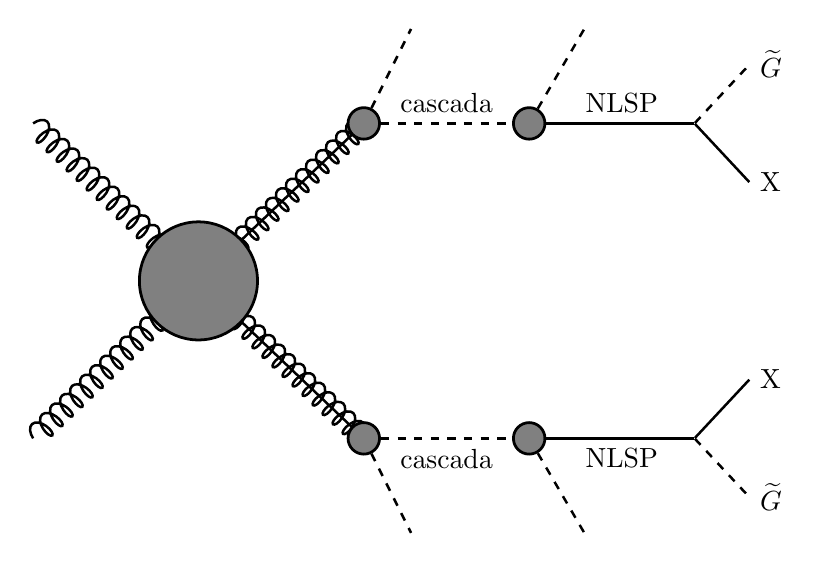
\begin{tikzpicture}

	\tikzset{
    		line/.style={line width=0.9},
    		dline/.style={dashed,line width=0.9},
  	}

	\definecolor{blue1}{HTML}{3F66BD}
	\definecolor{blue2}{HTML}{2C4784}

	\coordinate[vertex] (O) at (0,0);

	\coordinate[vertex] (C1) at (2.1, 2);
	\coordinate[vertex] (C2) at (2.1,-2);

	\coordinate[vertex] (N1_a) at (4.2, 2);
	\coordinate[vertex] (N2_a) at (4.2,-2);

	\coordinate[vertex] (N1_b) at (6.3, 2);
	\coordinate[vertex] (N2_b) at (6.3,-2);

	\coordinate[vertex] (G1) at (7, 2.75);
	\coordinate[vertex] (X1) at (7, 1.25);

	\coordinate[vertex] (G2) at (7,-2.75);
	\coordinate[vertex] (X2) at (7,-1.25);

	\draw[line,gluon] (-2.1,-2) -- (O);
	\draw[line,gluon] (-2.1, 2) -- (O);

	\draw[line] (O) -- (C1);
	\draw[line] (O) -- (C2);
	\draw[line,gluino] (O) -- (C1);
	\draw[line,gluino] (O) -- (C2);

	\draw[line] (4.0, 2) -- (N1_b) node[above, pos=.6] {NLSP};
	\draw[line] (4.0,-2) -- (N2_b) node[below, pos=.6] {NLSP};

	\draw[dline] (N1_b) -- (G1) node[right] {$\widetilde{G}$};
	\draw[line] (N1_b) -- (X1) node[right] {X};

	\draw[dline] (N2_b) -- (G2) node[right] {$\widetilde{G}$};
	\draw[line] (N2_b) -- (X2) node[right] {X};

    	\draw[black, line width=1, fill=gray] (O) circle (0.75cm); 

  	\draw[dline,fill=white] (C1) -- (N1_a) node[black,above,pos=.5] {cascada};
  	\draw[dline,fill=white] (C2) -- (N2_a) node[black,below,pos=.5] {cascada};

	\draw[dline] (C1) -- (2.7, 3.2);
	\draw[dline] (C2) -- (2.7,-3.2);
	\draw[dline] (N1_a) -- (4.9, 3.2);
	\draw[dline] (N2_a) -- (4.9,-3.2);


	\draw[black, line width=1,fill=gray] (C1) circle (0.20cm);
	\draw[black, line width=1,fill=gray] (C2) circle (0.20cm);
	\draw[black, line width=1,fill=gray] (N1_a) circle (0.20cm);
	\draw[black, line width=1,fill=gray] (N2_a) circle (0.20cm);

\end{tikzpicture}
